% 2-bit saturating counter state machine (matches rtl/update_logic.v, STATE_BITS=2)
% Build: cd docs/diagrams && tectonic two_bit_fsm.tex
\documentclass[tikz,border=6pt]{standalone}
\usetikzlibrary{arrows.meta,automata,positioning,calc}
\begin{document}
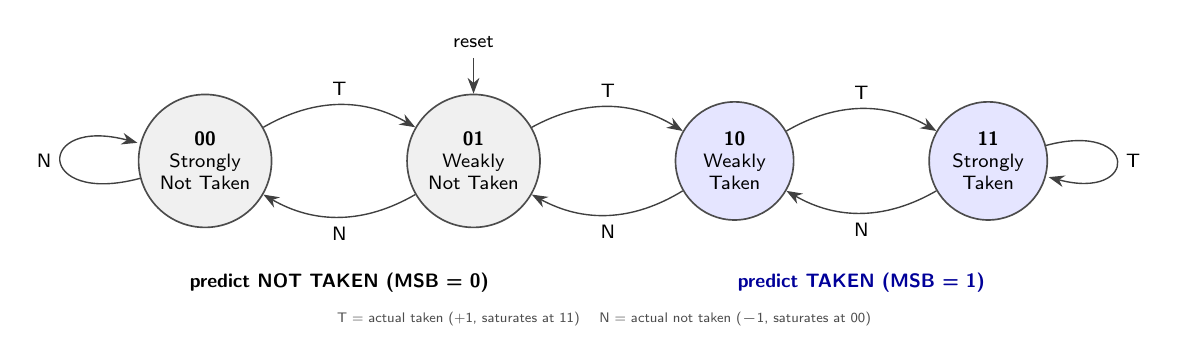
\begin{tikzpicture}[
  font=\sffamily\scriptsize, >={Stealth[length=2mm]}, node distance=17mm,
  st/.style={state, minimum size=15mm, align=center, draw=black!70, line width=0.6pt},
  every edge/.style={draw=black!75, line width=0.5pt}
]
\node[st, fill=black!6]  (s0) {\textbf{00}\\Strongly\\Not Taken};
\node[st, fill=black!6, initial above, initial text={reset}, right=of s0] (s1) {\textbf{01}\\Weakly\\Not Taken};
\node[st, fill=blue!10, right=of s1] (s2) {\textbf{10}\\Weakly\\Taken};
\node[st, fill=blue!10, right=of s2] (s3) {\textbf{11}\\Strongly\\Taken};

\path[->]
  (s0) edge[bend left=30] node[above]{T} (s1)
  (s1) edge[bend left=30] node[above]{T} (s2)
  (s2) edge[bend left=30] node[above]{T} (s3)
  (s3) edge[loop right]   node[right]{T} (s3)
  (s3) edge[bend left=30] node[below]{N} (s2)
  (s2) edge[bend left=30] node[below]{N} (s1)
  (s1) edge[bend left=30] node[below]{N} (s0)
  (s0) edge[loop left]    node[left]{N} (s0);

\node[below=13mm of $(s0)!0.5!(s1)$, font=\sffamily\scriptsize\bfseries] {predict NOT TAKEN (MSB = 0)};
\node[below=13mm of $(s2)!0.5!(s3)$, font=\sffamily\scriptsize\bfseries, text=blue!60!black] {predict TAKEN (MSB = 1)};
\node[below=18mm of $(s1)!0.5!(s2)$, font=\sffamily\tiny, text=black!70] {T = actual taken (+1, saturates at 11) \quad N = actual not taken ($-$1, saturates at 00)};
\end{tikzpicture}
\end{document}
